\documentclass[a4paper]{article}
\usepackage{amsmath,amssymb,algorithmic,booktabs,bm,caption,cases,csvsimple,enumerate,float,geometry,graphicx,indentfirst,makecell,multirow,setspace,tabularx,titlesec}
\captionsetup[figure]{labelsep=period}
\captionsetup[table]{labelsep=period}
\geometry{left=3.5cm,right=3.5cm,top=3.3cm,bottom=3.3cm}
\renewcommand\thesection{\arabic{section}}
\setlength{\parindent}{2em}
\begin{document}
\begin{center}
\huge
\textbf{VE320\\Intro to Semiconductor Devices\\}
\Large
\vspace{30pt}
\uppercase{Homework 1}\\
\vspace{5pt}\today\\
\vspace{5pt}
Yihua Liu 518021910998
\vspace{5pt}
\rule[-10pt]{.97\linewidth}{0.05em}
\end{center}

1.
$$E=h\nu$$
$$\nu=\frac{c}{\lambda}$$
Thus,
$$\lambda=\frac{hc}{E}$$
The maximum wavelength of light for the photoelectric emission of electrons for gold is:
$$\lambda_\text{max}=2.53\times10^{-7}\ \text{m}$$
The maximum wavelength of light for the photoelectric emission of electrons for cesium is:
$$\lambda_\text{max}=6.53\times10^{-7}\ \text{m}$$

2.

(a)
$$p=mv=\frac{h}{\lambda}$$
$$\lambda=5.5\times10^{-7}\ \text{m}$$
Thus, the electron momentum is
$$p=\frac{h}{\lambda}=1.20\times10^{-27}\ \text{kg}\cdot\text{m/s}$$
The electron velocity is
$$v=\frac{h}{m\lambda}=1.32\times10^3\ \text{m/s}$$

(b)
$$\lambda=5.5\times10^{-7}\ \text{m}$$
Thus, the electron momentum is
$$p=\frac{h}{\lambda}=1.51\times10^{-27}\ \text{kg}\cdot\text{m/s}$$
The electron velocity is
$$v=\frac{h}{m\lambda}=1.65\times10^3\ \text{m/s}$$

(c) Yes, the momentum of the photon is equal to the momentum of the electron.

3.

(a) Simple cubic\\
(i) (100) The surface density of atoms is
$$\frac{10^{-4}}{(4.50\times10^{-10})^2}=4.94\times10^{14}\ \text{cm}^{-2}$$
(ii) (110) The surface density of atoms is
$$\frac{10^{-4}}{\sqrt{2}\times(4.50\times10^{-10})^2}=3.49\times10^{14}\ \text{cm}^{-2}$$
(iii) (111) The surface density of atoms is
$$\frac{\frac{1}{2}\times10^{-4}}{\frac{\sqrt{2}}{2}\times\frac{\sqrt{6}}{2}\times(4.50\times10^{-10})^2}=2.85\times10^{14}\ \text{cm}^{-2}$$

(b) Body-centered cubic\\
(i) (100) The surface density of atoms is
$$\frac{10^{-4}}{(4.50\times10^{-10})^2}=4.94\times10^{14}\ \text{cm}^{-2}$$
(ii) (110) The surface density of atoms is
$$\frac{2\times10^{-4}}{\sqrt{2}\times(4.50\times10^{-10})^2}=6.98\times10^{14}\ \text{cm}^{-2}$$
(iii) (111) The surface density of atoms is
$$\frac{\frac{1}{2}\times10^{-4}}{\frac{\sqrt{2}}{2}\times\frac{\sqrt{6}}{2}\times(4.50\times10^{-10})^2}=2.85\times10^{14}\ \text{cm}^{-2}$$

(c) Face-centered cubic\\
(i) (100) The surface density of atoms is
$$\frac{2\times10^{-4}}{(4.50\times10^{-10})^2}=9.88\times10^{14}\ \text{cm}^{-2}$$
(ii) (110) The surface density of atoms is
$$\frac{2\times10^{-4}}{\sqrt{2}\times(4.50\times10^{-10})^2}=6.98\times10^{14}\ \text{cm}^{-2}$$
(iii) (111) The surface density of atoms is
$$\frac{2\times10^{-4}}{\frac{\sqrt{2}}{2}\times\frac{\sqrt{6}}{2}\times(4.50\times10^{-10})^2}=1.14\times10^{15}\ \text{cm}^{-2}$$

4. The average electron energy is
$$E=\frac{3kT}{2}=6.21\times10^{-21}\ \text{J}=3.88\times10^{-2}\ \text{eV}$$
The average electrons momentum is
$$p=\sqrt{2m_eE}=\sqrt{3m_ekT}=1.06\times10^{-25}\ \text{kg}\cdot\text{m/s}$$
The de Broglie wavelength is
$$\lambda=\frac{h}{p}=\frac{h}{\sqrt{3m_ekT}}=6.23\times10^{-9}\ \text{m}$$

5.

(a) The energy levels are
$$E_n=\frac{n^2\pi^2\hbar^2}{2ma^2}$$
The width
$$a=10^{-9}\ \text{m}$$
The first three energy levels are
$$E_1=\frac{\pi^2\hbar^2}{2m_ea^2}=6.02\times10^{-20}\ \text{J}=0.376\ \text{eV}$$
$$E_2=\frac{4\pi^2\hbar^2}{2m_ea^2}=2.41\times10^{-19}\ \text{J}=1.504\ \text{eV}$$
$$E_3=\frac{9\pi^2\hbar^2}{2m_ea^2}=5.42\times10^{-19}\ \text{J}=3.384\ \text{eV}$$

(b) The wavelength of a photon that might be emitted is
$$\lambda=\frac{hc}{E_3-E_2}=\frac{8cm_ea^2}{5h}=6.59\times10^{-7}\ \text{m}$$

6.

(a) The de Broglie wavelength of an electron is
$$\lambda=8.5\times10^{-9}\ \text{m}$$
The electron momentum is
$$p=\frac{h}{\lambda}=7.80\times10^{-26}\ \text{kg}\cdot\text{m/s}$$
The electron velocity is
$$v=\frac{p}{m_e}=\frac{h}{m_e\lambda}=8.56\times10^{4}\ \text{m/s}$$
The electron energy is
$$E=\frac{p^2}{2m_e}=\frac{h^2}{2m_e\lambda^2}=3.34\times10^{-21}\ \text{J}=2.08\times10^{-2}\ \text{eV}$$

(b) The velocity of the electron is
$$v=8\times10^3\ \text{m/s}$$
The electron energy is
$$E=\frac{1}{2}m_ev^2=2.92\times10^{-23}\ \text{J}=1.82\times10^{-4}\ \text{eV}$$
The electron momentum is
$$p=m_ev=7.29\times10^{-27}\ \text{kg}\cdot\text{m/s}$$
The de Broglie wavelength is
$$\lambda=\frac{h}{m_ev}=9.09\times10^{-8}\ \text{m}=909\ \text{\AA}$$

7. Since
$$\int_{-\infty}^\infty|\Psi(x,t)|^2\mathrm{d}x=1,$$
we have
$$\int_{-\infty}^{-1}|\Psi(x,t)|^2\mathrm{d}x+\int_{-1}^3|\Psi(x,t)|^2\mathrm{d}x+\int_3^\infty|\Psi(x,t)|^2\mathrm{d}x=1$$
thus,
$$\int_{-\infty}^{-1}0\mathrm{d}x+\int_{-1}^3|A(\cos{(\frac{\pi x}{2})})e^{-j\omega t}|^2\mathrm{d}x+\int_3^\infty0\mathrm{d}x=1.$$
Then,
$$\int_{-1}^3A^2\cos^2{(\frac{\pi x}{2})}\mathrm{d}x=1$$
Since
$$\int\cos^2{(\frac{\pi x}{2})}\mathrm{d}x=\frac{x}{2}+\frac{\sin{\pi x}}{2\pi},$$
we have
$$2A^2=1.$$
Therefore,
$$A=\frac{\sqrt{2}}{2}.$$

8.

(a) The time-independent Schrodinger's wave equation is
\begin{equation}
    \frac{-\hbar^2}{2m}\cdot\frac{1}{\psi(x)}\cdot\frac{\partial^2\psi(x)}{\partial x^2}+V(x)=E.
\end{equation}
or
\begin{equation}
    -\frac{\hbar^2}{2m}\frac{\partial^2\psi}{\partial x^2}+V(x)\psi=E\psi.
\end{equation}
Condition: for $x<0$, $V(x)=V_0$, so
$$-\frac{\hbar^2}{2m}\frac{\partial^2\psi}{\partial x^2}=(E-V_0)\psi.$$
Thus, the general solution of $\psi$ is
$$\psi_1(x)=Ae^{-jk_1x}+Be^{jk_1x}.$$
Condition: for $0\leq x\leq a$, $V(x)=0$, so
$$-\frac{\hbar^2}{2m}\frac{\partial^2\psi}{\partial x^2}=E\psi.$$
Thus, the general solution of $\psi$ is
$$\psi_2(x)=Ce^{-jk_2x}+De^{jk_2x}.$$
Condition: for $x>a$, $V(x)=\infty$, so the equation
$$-\frac{\hbar^2}{2m}\frac{\partial^2\psi}{\partial x^2}+V(x)\psi=E\psi$$
has the general solution of $\psi$ of
$$\psi_3(x)=0.$$
Solving the equations, we have
$$k_1=\sqrt{\frac{2m(E-V_0)}{\hbar^2}}$$
$$k_2=\sqrt{\frac{2mE}{\hbar^2}}$$
Besides, later we would calculate the integral of $\psi_1$ and note that $\psi_1(x)<\infty$ when $x<a$, so $A=0$, then $\psi_1(x)=Be^{jk_1x}$.

In addition, later we would calculate the integral of $\psi_2$ and need to use Eq. (2.29) in the textbook as an alternative particular form of solution to the Schrodinger's equation:
$$\psi_2(x)=A_1\cos{k_2x}+A_2\sin{k_2x}.$$

Therefore, the wave solutions that apply in each region are
$$\psi(x)=\left\{\begin{array}{rcl}
    Be^{j\sqrt{\frac{2m(E-V_0)}{\hbar^2}}x},&&x<0\\
    A_1\cos{\sqrt{\frac{2mE}{\hbar^2}}x}+A_2\sin{\sqrt{\frac{2mE}{\hbar^2}}x},&&0\leq x\leq a\\
    0,&&x>a
\end{array}
\right.$$

(b) Applying the boundary conditions:\\
\textcircled{1} at $x=0$, $\psi_1=\psi_2$, $B=A_2$;\\
\textcircled{2} at $x=0$, $\frac{\partial\psi_1}{\partial x}=\frac{\partial\psi_2}{\partial x}$, $jk_1B=k_2A_1$;\\
\textcircled{3} at $x=a$, $\psi_2=\psi_3=0$, $A_1\cos{k_2x}+A_2\sin{k_2x}=0\Rightarrow A_2=-A_1\tan{k_2a};$\\
\textcircled{4} $\int_{-\infty}^\infty|\psi|^2\mathrm{d}x=\int_{-\infty}^0|\psi_1|^2\mathrm{d}x+\int_0^a|\psi_2|^2\mathrm{d}x+\int_a^\infty|\psi_3|^2\mathrm{d}x=\int_{-\infty}^0\psi_1\psi_1^*\mathrm{d}x+\int_0^a\psi_2\psi_2^*\mathrm{d}x=1$.\\
% Since $(Ae^{-jk_1x}+Be^{jk_1x})((Ae^{-jk_1x}+Be^{jk_1x})=A^2+B^2+AB(e^{-2jk_1x}+e^{2jk_1x})$, $\int_{-\infty}^0|\psi_1|^2\mathrm{d}x=(A^2+B^2)x+\frac{jAB}{2k_1}(e^{-2jk_1x}+e^{2jk_1x})|_{-\infty}^0$ is finite, $A^2+B^2=0$, $AB=0$, thus $A=B=0$.

We would assume that the wave function solution $\psi(x)$ is a real function, then $\psi(x)=\psi^*(x)$. To prove $\psi(x)$ can be chosen to be real, consider Eq. (1) and (2), we have
\begin{equation}
    \frac{\hbar^2}{2m}\psi''+(E-V(x))\psi=0.
\end{equation}
Since $(\psi'')^*=(\psi^*)''$, the complex conjugation of Eq. (3) is
$$\frac{\hbar^2}{2m}(\psi^*)''+(E-V(x))\psi^*=0.$$
By superposition, we can derive the real and the imaginary parts of $\psi$ that are real solutions to the equation:
$$\psi_{re}=\frac{1}{2}(\psi+\psi^*),\qquad\psi_{im}=\frac{1}{2j}(\psi-\psi^*).$$

Hence, we have proved that solution $\psi(x)$ of the time-independent Schrodinger equation can always be chosen to be real.

Using the assumption above, the integral becomes
\[
    \begin{aligned}
        \int_{-\infty}^\infty|\psi|^2\mathrm{d}x
        &=\int_{-\infty}^0B^2e^{2jk_1x}+\int_0^a(A_1\cos{k_2x}+A_2\sin{k_2x})^2\mathrm{d}x\\
        &=\frac{B^2}{2j}e^{2jk_1x}\bigg|_{-\infty}^0+\frac{(2k_2x+\sin{2k_2x})A_1^2-2\cos{2k_2x}A_1A_2+(2k_2x-\sin{2k_2x})A_2^2}{4k}\bigg|_0^a\\
        &=\frac{B^2}{2j}+\frac{(2k_2a+\sin{2k_2a})A_1^2+2(1-\cos{2k_2a})A_1A_2+(2k_2a-\sin{2k_2a})A_2^2}{4k}\\
        &=1.
    \end{aligned}
\]

Since only three constants remain unknown, we only need three equations. Therefore, the set of equations that result from applying the boundary conditions are
\begin{equation}
    B=A_2
\end{equation}
\begin{equation}
    jk_1B=k_2A_1
\end{equation}
\begin{equation}
    A_2=-A_1\tan{k_2a}
\end{equation}

(c) Using the set of equations above in (b), combining Eq. (4) and (5),
\begin{equation}
    A_1=\frac{jk_1A_2}{k_2}.
\end{equation}
Combining Eq. (6) and (7),
$$A_2=-\frac{jk_1A_2}{k_2}\tan{k_2a},$$
then,
$$-\tan{k_2a}=\frac{jk_2}{k_1}.$$
Thus,
$$\sqrt{\frac{E}{V_0-E}}=-\tan{\bigg(\sqrt{\frac{2mE}{\hbar^2}}a\bigg)}$$
The solutions of $E$ as the intersections comprising a discrete set. For example, suppose $V_0=10$ eV and $a=10^{-9}$ m,
\begin{figure}[H]
    \begin{center}
        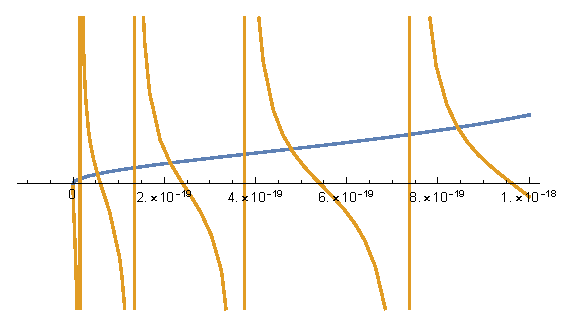
\includegraphics[width=0.8\textwidth]{1-8(c).eps}
    \end{center}
    \caption{Graph of $\sqrt{\frac{E}{V_0-E}}$ and $-\tan{\big(\sqrt{\frac{2mE}{\hbar^2}}a\big)}$.}
\end{figure}
Therefore, the energy levels of the electron are quantized.
\end{document}